

\documentclass[12pt, a4paper]{article}

\raggedbottom

\RequirePackage[l2tabu, orthodox]{nag}

\usepackage[top=20mm,bottom=20mm,left=25mm,right=25mm]{geometry}

\usepackage{showkeys}

\usepackage{amsmath,amssymb,amsfonts}

\usepackage{centernot}

\usepackage{underbracket}

\usepackage[nottoc]{tocbibind}

\usepackage{pgf}
\usepackage{tikz}

\usepackage{multirow}

\usepackage{pgf}
\usepackage{tikz}
%\usetikzlibrary{calc}

\usepackage{xcolor}

% Syntax: \colorboxed[<color model>]{<color specification>}{<math formula>}
\newcommand*{\colorboxed}{}
\def\colorboxed#1#{%
  \colorboxedAux{#1}%
}
\newcommand*{\colorboxedAux}[3]{%
  % #1: optional argument for color model
  % #2: color specification
  % #3: formula
  \begingroup
    \colorlet{cb@saved}{.}%
    \color#1{#2}%
    \boxed{%
      \color{cb@saved}%
      #3%
    }%
  \endgroup
}

\usepackage[most]{tcolorbox}

\tcbset{
    frame code={}
    center title,
    left=0pt,
    right=0pt,
    top=0pt,
    bottom=0pt,
    colback=green!15,
    colframe=white,
    % width=\dimexpr\textwidth\relax,
    enlarge left by=0mm,
    % boxsep=5pt,
    arc=0pt,outer arc=0pt,
    breakable,
    }

\usepackage{amsthm}

\usepackage{thmtools}
%\usepackage{thm-restate}   This package does not interact very smoothly with \theoremstyle and \listoftheorems

\newtheoremstyle{break}{9pt}{9pt}{\itshape}{}{\bfseries}{}{\newline}{}
\theoremstyle{break}    

\newtheorem{exo}{Exercise}[section]
\newtheorem{hyp}[exo]{Axiom}
\newtheorem{res}[exo]{Result}
\newtheorem{defn}[exo]{Definition}

\makeatletter
\def\ll@exo{%
  \protect\numberline{\csname the\thmt@envname\endcsname}%
  \ifx\@empty\thmt@shortoptarg
    \thmt@thmname
  \else
    \thmt@shortoptarg
  \fi}
\def\l@thmt@exo{} 
\makeatother

\usepackage[colorlinks=true,linktoc=all,linkcolor=black,citecolor=red,urlcolor=blue,backref=page]{hyperref}

\usepackage{etoolbox}
\makeatletter
\patchcmd{\BR@backref}{\newblock}{\newblock(}{}{}
\patchcmd{\BR@backref}{\par}{)\par}{}{}
\makeatother

\renewcommand{\arraystretch}{1.3}

\title{\bfseries Exactly solvable two-dimensional \\ conformal field theories}

\author{Sylvain Ribault \vspace{2mm}
\\
{\normalsize CEA Saclay, Institut de Physique Th\'eorique}
 \\
 {\footnotesize \ttfamily sylvain.ribault@ipht.fr }
}

\begin{document}


\maketitle


\begin{abstract}
This course will introduce two-dimensional CFT in the bootstrap approach, and sketch the known exactly solvable CFTs with no extended chiral symmetry.
\begin{itemize}
 \item The Virasoro algebra, its representations, Ward identities, fusion rules.
 \item (Generalized) minimal models, Liouville theory, logarithmic minimal models, the $O(n)$ model and more general loop models. Taking limits in the central charge and/or in conformal dimensions. 
 \item Conformal bootstrap methods, analytic and numerical. Generic and degenerate conformal blocks. Crossing symmetry equations and their solutions. 
 \item Exactly known structure constants. Analytic properties of correlation functions. 
\end{itemize}
\end{abstract}

\vspace{5mm}


\textit{
Could make life easier by renouncing logarithms. But they appear naturally when taking limits, and are in principle needed for solving the $O(n)$ model.}

\clearpage

\tableofcontents

\hypersetup{linkcolor=blue}

\numberwithin{equation}{section}
%\setcounter{secnumdepth}{2}
%\setcounter{tocdepth}{2}
\setcounter{section}{-1}

\section{Introduction}

Sketch map of CFTs according to symmetry: deg. fields, no deg. fields, local conf. sym, global conf. sym.

CFTs that are exactly solvable with known methods = bootstrap, analytic and numerical. Only Virasoro. Do not characterize with twist gap, as symmetry cannot be inferred from spectrum: chiral symmetry fields might be absent from spectrum. Also, affine abelian symmetry can be present in spectrum but absent in interactions. (Is there a strong statement that unitary CFTs do not have these pathologies?)

Forget Coulomb gas, a dead end. For correl fct, applies only if we have two deg. fields? But used to find spectrum of $O(n)$ etc. Larger symmetry allows many generalizations, but tend to be always more complicated. (Liouville not solved from WZW, quite the opposite.) No modular bootstrap. 

Exact solution means analytic expression for three-point structure constants. Here: CFTs that are presumed to be solvable, not necessarily solved. 

Focus on correl fct: no modular bootstrap, no KPZ. These methods are efficient at getting the spectrum but we can get it otherwise. 

This review: only necessary calculations. Derive the recursion for blocks? hard part is coef $R_{r,s}$ but it obeys simple shift equations. Rewrite it in terms of Upsilon functions, and somehow derive it from Liouville theory! But cancellation of double poles hard to argue? And need to determine sign, since we get square of $R_{r,s}$. We can choose any value of the continuous parameters including $c$, but is there a value that makes $R_{r,s}$ simple enough? And what about the $\Delta\to\infty$ prefactors? See Yin et al? See Appendix D of \cite{msz15} for the pillow geometry that underlies the variable $q$.

Use low central charge notations ($\beta$ not $b$) because more examples. Rare are solved CFTs with large $c$.

define somewhere \textbf{extended chiral algebra}

Nothing about unitarity?

Relation with \cite{rib16}.

Words in bold are defined.

\subsection*{Acknowledgements}


%\end{tcolorbox}

\section{Basic structures}

In this section we will introduce the basic structures of conformal field theory: conformal symmetry, fields, and operator product expansions. In particular, we will focus on the two ingredients of exact solvability: \textit{local} conformal symmetry and \textit{degenerate} fields. 

\subsection{The Virasoro algebra and its representations}

\subsubsection{The Virasoro algebra}

Let us consider the Riemann sphere $\overline{\mathbb{C}}=\mathbb{C}\cup \{\infty\}$, equipped with the metric $ds^2 = dzd\bar z$. By definition, a conformal transformation of a Riemannian manifold is a transformation that preserves angles. On any open subset of the Riemann sphere, a map $z\to f(z)$ is conformal if and only if it is holomorphic. It is indeed straightforward to show that any holomorphic map is conformal,
because it transforms the metric into itself, up to a scalar factor: 
\begin{align}
 dzd\bar z\to dfd\bar f = |f'(z)|^2 dzd\bar z\ .
\end{align}
Let us define the \textbf{Witt algebra} as the Lie algebra of infinitesimal conformal transformations on $\mathbb{C}^*= \mathbb{C}-\{0\}$. This algebra describes local conformal symmetry for quantum field theory on the Riemann sphere, as can be argued in two alternative ways:
\begin{itemize}
 \item Transformations need not be defined at $z=\infty$ because they are local, and can be singular at $z=0$ if we insert a field at that point.
 \item Holomorphic functions on $\mathbb{C}^*$ are equivalent to holomorphic functions on a neighbourhood of the circle $|z|=1$, which can be interpreted as a Euclidean time slice where the states of our theory live. 
\end{itemize}
The Witt algebra is infinite-dimensional, with the basis 
\begin{align}
 \left(\ell_n\right)_{n\in\mathbb{Z}}  \quad \text{with} \quad \ell_n = -z^{n+1}\frac{\partial}{\partial z}\ ,
 \label{lpz}
\end{align}
and the commutation relations 
\begin{align}
 [\ell_n,\ell_m] = (n-m)\ell_{m+n}\ .
\end{align}
The generators of the Witt algebra include the translation generator $\ell_{-1} = -\frac{\partial}{\partial z}$, and the dilation generator $\ell_0 = -z\frac{\partial}{\partial z}$. In fact, $(\ell_{-1},\ell_0,\ell_1)$ generate the infinitesimal conformal transformations on the full Riemann sphere.
The corresponding Lie group is the group of global conformal transformations $PSL_2(\mathbb{C})$, whose elements act as 
\begin{align}
 z \mapsto \frac{az+b}{cz+d}\quad , \quad (a,b,c,d\in \mathbb{C},\ ad-bc\neq 0)\ .
\end{align}
Now, in a quantum theory, symmetries act projectively on states. And projective representations of an algebra are equivalent to representations of that algebra's central extension. Therefore, the algebra that describes local conformal transformations in conformal field theory is the Witt algebra's central extension, called the Virasoro algebra. The \textbf{Virasoro algebra} $\mathfrak{V}$ has generators $(L_n)_{n\in\mathbb{Z}}$ that correspond to the Witt algebra generators, plus a central generator $\mathbf 1$. The commutation relations are 
 \begin{align}
  [\mathbf 1, L_n] = 0 \quad , \quad \boxed{[L_n,L_m] = (n-m)L_{n+m} +\frac{c}{12}(n-1)n(n+1)\delta_{n+m,0}\mathbf 1} \ .
  \label{vir}
 \end{align}
 The \textbf{central charge} $c\in\mathbb{C}$ is a fundamental parameter not only of the Virasoro algebra, but also of any conformal field theory built on that algebra. 

\subsubsection{Highest-weight representations}

In a conformal field theory, the spectrum is a representation of the Virasoro algebra, and can be decomposed into indecomposable representations. But which indecomposable representations are physically relevant? To answer this question, we will focus on the properties of the generator $L_0$ of the Virasoro algebra. Conceptually, this is because $L_0$ can be interpreted as the energy operator. Technically, since $L_0$ generates dilations, it controls the convergence of operator product expansions, as we will see in Section \ref{sec:ope}. More specifically, a necessary condition for convergence is that the eigenvalues of $L_0$ be bounded from below in any indecomposable representation. We will always work under this assumption.

%We now make the further technical assumption that $L_0$ be diagonalizable. This assumption holds in Liouville theory and minimal models, and also in many representations that appear in other solvable CFTs. However, it does not hold in the logarithmic representations of Section \ref{sec:log}. 

The eigenvalues of $L_0$ are called \textbf{conformal dimensions}. Under the action of the Virasoro generator $L_n$, the conformal dimension decreases by $n$:
\begin{align}
 L_0|v\rangle = \Delta|v\rangle \quad \Rightarrow\quad  L_0 L_n|v\rangle = L_nL_0|v\rangle + [L_0, L_n] |v\rangle  = (\Delta-n)L_n|v\rangle \ .
\end{align}
In an indecomposable representation $\mathcal{R}$, the $L_0$-eigenstate $|v\rangle$ with the lowest eigenvalue $\Delta$ must therefore be annihilated by $L_{n>0}$:
\begin{align}
  L_0 |v\rangle = \Delta |v\rangle \quad , \quad L_{n>0} |v\rangle = 0\ .
 \end{align}
Any nonzero state that obeys these conditions is called a \textbf{primary state}, even if its eigenvalue is not the smallest. Any state of the type $\prod_{i=1}^k L_{-n_i} |v\rangle$ with $k\in\mathbb{N}$ and $ 0<n_1\leq \dots \leq n_k$ is called a \textbf{descendant state} of that primary state. Let  $N=\sum_{i=1}^k n_i \in\mathbb{N}$ be the  \textbf{level} of that state, then its conformal dimension is $\Delta+N$. By extension, a linear combination of descendant states is also called a descendant state. 

A primary state $|v\rangle \in \mathcal{R}$ generates a subrepresentation $\mathcal{R}_{|v\rangle}\subset\mathcal{R}$, which is the space of its descendant states. The states $\left\{\prod_{i=1}^k L_{-n_i} |v\rangle\right\}_{0<n_1\leq \dots \leq n_k}$ generate $\mathcal{R}_{|v\rangle}$. If they are linearly independent, then $\mathcal{R}_{|v\rangle}$ is called the \textbf{Verma module} $\mathcal{V}_\Delta$. More generally, $\mathcal{R}_{|v\rangle}$ is a quotient of $\mathcal{V}_\Delta$ by a subrepresentation (trivial or not): such quotients are called \textbf{highest-weight representations}. In such a representation, $L_0$ is diagonalizable. 
Let us sketch a Verma module by displaying all its basis states up to the level $N=3$, with arrows representing the action of the Virasoro generators $L_{-1},L_{-2},L_{-3}$:
\begin{align}
 \begin{tikzpicture}[scale = .25, baseline=(current  bounding  box.center)]
  \draw[-latex, very thick] (20, 0) -- (20, -21) node [right] {$N$};
  \foreach \x in {0, ..., 3}
  {
  \draw [dotted] (-20, {-6*\x}) -- (20, {-6*\x}) node [right] {${\x}$};
  }
  \node[fill = white] at (0, 0) (0) {$|v\rangle$};
  \node[fill = white] at (-4,-6) (1) {$L_{-1}|v\rangle$};
  \node[fill = white] at (-8, -12) (11) {$L_{-1}^2|v\rangle$};
  \node[fill = white] at (-12, -18) (111) {$L_{-1}^3|v\rangle$};
  \node[fill = white] at (0,-12) (2) {$L_{-2}|v\rangle$};
  \node[fill = white] at (0,-18) (12) {$L_{-1}L_{-2}|v\rangle$};
  \node[fill = white] at (8,-18) (3) {$L_{-3}|v\rangle$};
  \draw[-latex] (0) -- (1);
  \draw[-latex] (1) -- (11);
  \draw[-latex] (11) -- (111);
  \draw[-latex] (0) -- (2);
  \draw[-latex] (0) -- (3);
  \draw[-latex] (2) -- (12);
 \end{tikzpicture}
\end{align}

\subsubsection{Null vectors of Verma modules}

In a representation of the Virasoro algebra, we define a \textbf{null vector} or singular vector as a primary state that is a descendant of another primary state. Null vectors play an important structural role: a highest-weight representation is irreducible if and only if it has no null vector. 

Let us look for null vectors in the Verma module $\mathcal{V}_\Delta$. This can be done level by level, starting with level $1$. That level is generated by a single state $L_{-1}|v\rangle$. To determine whether that state is primary, we take $n\geq 1$ and compute 
\begin{align}
L_n L_{-1}|v\rangle = [L_n, L_{-1}] |v\rangle = (n+1) L_{n-1}|v\rangle = 
\left\{\begin{array}{ll} 0 &  \quad \text{if } n\geq 2\ , \\ 2\Delta |v\rangle & \quad \text{if } n = 1\ . \end{array}\right. 
\end{align}
Therefore, $\mathcal{V}_\Delta$ has a null vector at level $1$ if and only if $\Delta=0$. Next, consider the case of level $2$, where we write states as 
\begin{align}
 |\chi\rangle = \left(a_{1,1} L_{-1}^2 + a_2 L_{-2}\right) |v\rangle\ ,
\end{align}
where $a_{1,1}$ and $a_2$ are complex coefficients. It is easy to show that $L_{n\geq 3}|\chi\rangle=0$, and we compute 
\begin{align}
 L_1|\chi\rangle &= \left((4\Delta+2)a_{1,1} + 3a_2\right) L_{-1}|v\rangle\ ,
\\
L_2 |\chi \rangle &= \left(6\Delta a_{1,1}+(4\Delta+\tfrac12 c) a_2\right)|v\rangle\ .
\end{align}
Therefore, the condition $L_1|\chi\rangle=L_2 |\chi \rangle=0$ for $|\chi\rangle$ to be a null vector boil down to a system of two linear equations for the coefficients $(a_{1,1},a_2)$. The vanishing of that system's determinant determines the conformal dimension $\Delta$ as a function of the central charge $c$,
\begin{align}
 \Delta = \frac{1}{16}\left( 5-c\pm\sqrt{(c-1)(c-25)} \right) \ .
 \label{dpm}
\end{align}
Solving CFTs will lead to fairly complicated formulas, which would become even more complicated if we tolerated a square root at this early and elementary stage.
To get rid of the square root, we rewrite the central charge in terms a the parameter $\beta$ such that 
\begin{align}
 \boxed{c = 1- 6\left(\beta - \beta^{-1}\right)^2 } \ .
\end{align}
Then the conformal dimensions \eqref{dpm} of the two Verma modules that have null vectors become 
$
 \Delta = -\frac12 + \frac34\beta^{\pm 2}
$. The price to pay for this simplification is that the four values $\beta,-\beta,\beta^{-1},-\beta^{-1}$ all correspond to the same central charge. 

More generally, there is an infinite family of conformal dimensions $(\Delta_{(r, s)})_{r,s\in\mathbb{N}^*}$ such that $\mathcal{V}_{\Delta_{(r, s)}}$ has a null vector $|\chi_{\langle r,s\rangle}\rangle = L_{\langle r,s\rangle} |v\rangle$ at level $N=rs$. Let us summarize the cases $N=1,2$ in these notations:
\begin{align}
\begin{array}{|c|c|c|c|}
\hline 
N & (r, s) & \Delta_{(r, s)} &  L_{\langle r,s\rangle} 
\\
\hline\hline
1 & (1, 1) & 0 &  L_{-1}
\\
\hline
\multirow{2}{*}{2} & 
(2, 1) & -\frac12 + \frac34 \beta^{2}  & L_{-1}^2 -\beta^{2} L_{-2}
\\
\cline{2-4}
& (1, 2) & -\frac12 + \frac34 \beta^{-2} & L_{-1}^2 -\beta^{-2} L_{-2} 
\\
\hline
\end{array}
\label{eq:ars}
\end{align}
To write $\Delta_{(r, s)}$ for any $r,s\in\mathbb{N}^*$, we rewrite the conformal dimension in terms of the momentum $P$ defined by 
\begin{align}
 \boxed{\Delta = \frac{c-1}{24} + P^2}\ .
 \label{dp}
\end{align}
The conformal dimension is invariant under the \textbf{reflection} $P\to -P$. The dimensions $\Delta_{(r, s)}$ correspond to the momentums 
\begin{align}
 \boxed{P_{(r, s)} = \frac12\left(r\beta -s\beta^{-1}\right)}\ ,
 \label{prs}
\end{align}
and it follows that the null vector $|\chi_{\langle r,s\rangle}\rangle$ is a primary state of dimension
\begin{align}
 \Delta_{(r, s)} + rs = \Delta_{(r, -s)}\ , 
 \label{drms}
\end{align}
We will provide a derivation of $P_{(r, s)}$ using operator product expansions in Section \ref{sec:dope}. On the other hand, the expressions for the null vectors $|\chi_{\langle r,s\rangle}\rangle$ themselves are complicated and not particularly useful. 

For $\beta^2\in\mathbb{C}-\mathbb{Q}$, the Verma module $\mathcal{V}_\Delta$ has a null vector if and only if $\Delta=\Delta_{(r, s)}$ for some $r,s\in\mathbb{N}^*$, in which case it has only one null vector. For $\beta^2\in\mathbb{Q}$ however, a Verma module can have several null vectors. If $\beta^2 = \frac{q}{p}$ with $p,q$ coprime integers, we indeed have the identity
\begin{align}
 \Delta_{(r+p,s+q)} = \Delta_{(r,s)}\ ,
 \label{rpsq}
\end{align}
which together with $\Delta_{(r,s)}=\Delta_{(-r,-s)}$ implies infinitely many coincidences of the type $\Delta_{(r,s)}=\Delta_{(r',s')}$. 
Whenever $r',s'>0$, the Verma module $\mathcal{V}_{\Delta_{(r,s)}}$ has a null vector $|\chi_{\langle r',s'\rangle}\rangle= L_{\langle r',s'\rangle} |v\rangle$. 
Moreover, if we apply the identity \eqref{rpsq} to the dimension $\Delta_{(r',-s')}$ \eqref{drms} of that null vector, we find that it is itself of the type $\Delta_{\langle r'',s''\rangle}$. If $r'',s''>0$, this leads to another null vector $L_{\langle r'',s''\rangle}L_{\langle r',s'\rangle} |v\rangle$. It turns out that all null vectors of Verma modules are of the type $L_{\langle r',s'\rangle} |v\rangle$ or $L_{\langle r'',s''\rangle}L_{\langle r',s'\rangle} |v\rangle$: in particular, $L_{\langle r''',s'''\rangle}L_{\langle r'',s''\rangle}L_{\langle r',s'\rangle} |v\rangle$ is of the type $L_{\langle r'''',s''''\rangle} |v\rangle$.

 Numbers of null vectors depend a lot on the sign of $\beta^2$. If $\beta^2<0$, then $\{\Delta_{(r, s)}\}_{r,s\in\mathbb{N}^*}$ is bounded from above, and Eq. \eqref{drms} implies that a Verma module can only have finitely many null vectors. If $\beta^2>0$, then by Eq. \eqref{rpsq} the existence of a null vector implies the existence of infinitely many others: 
\begin{align}
 \begin{array}{|c||c|c|c|}
  \hline 
  \text{Value of }\beta^2 & \mathbb{C}-\mathbb{Q} & \mathbb{Q}_{>0} & \mathbb{Q}_{<0}
  \\
  \hline 
  \#\text{null vectors in } \mathcal{V}_{\Delta_{(r, s)}} & 1 & \infty & \text{finite} 
  \\
  \hline 
 \end{array}
\end{align}
To illustrate the differences between these two cases, let us plot at each $(r,s)\in \{1,\dots, 10\}^2$ a dot whose size increases with 
$\Delta_{(r,s)}$, together with the vector $(p, q)$ of Eq. \eqref{rpsq} as a red arrow:
\begin{align}
 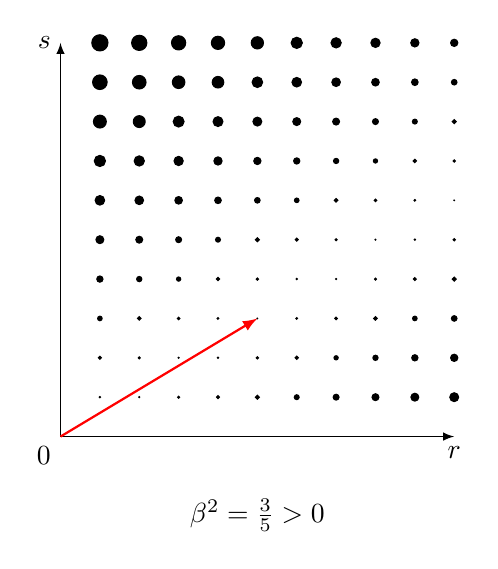
\begin{tikzpicture}[baseline=(base), scale = .5]
 \coordinate (base) at (0, 4);
  \draw[latex-latex] (0, 10) node [left] {$s$} -- (0, 0) node[below left] {$0$} -- (10, 0) node [below] {$r$};
  \draw[thick, red, -latex] (0, 0) -- (5, 3);
  \foreach \r in {1,...,10}{
  \foreach \s in {1,...,10}{
  %\pgfmathsetmacro{\mycol}{100-1.8*abs(3*\r-5*\s)}
  %\filldraw[black!\mycol] (\r, \s) circle [radius = 4pt];
  \pgfmathsetmacro{\myrad}{.2+.12*abs(3*\r-5*\s)}
  \filldraw (\r, \s) circle [radius = \myrad pt];
  }}
  \node at (5, -2) {$\beta^2 = \frac35>0$};
 \end{tikzpicture}
 \qquad \qquad
 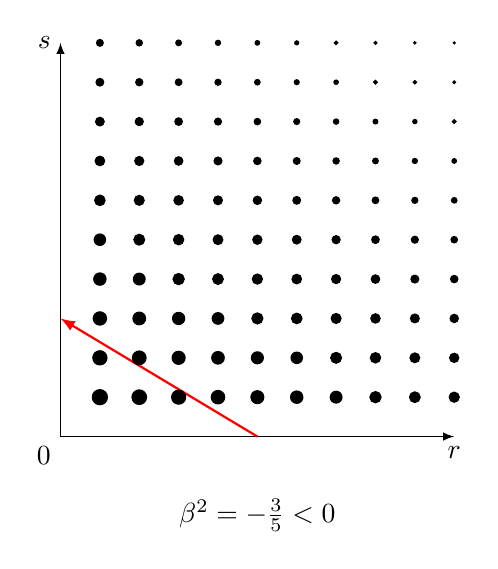
\begin{tikzpicture}[baseline=(base), scale = .5]
 \coordinate (base) at (0, 4);
  \draw[latex-latex] (0, 10) node [left] {$s$} -- (0, 0) node[below left] {$0$} -- (10, 0) node [below] {$r$};
  \draw[thick, red, -latex] (5, 0) -- (0, 3);
  \foreach \r in {1,...,10}{
  \foreach \s in {1,...,10}{
  %\pgfmathsetmacro{\mycol}{3*\r+5*\s}
  %\filldraw[black!\mycol] (\r, \s) circle [radius = 4pt];
  \pgfmathsetmacro{\myrad}{6-(3*\r+5*\s)/15}
  \filldraw (\r, \s) circle [radius = \myrad pt];
  }}
  \node at (5, -2) {$\beta^2 = -\frac35<0$};
 \end{tikzpicture}
\end{align}

\subsubsection{Vanishing and non-vanishing null vectors}

When a representation $\mathcal{R}$ has a null vector $|\chi\rangle=L|v\rangle$, this allows us to define a quotient representation $\frac{\mathcal{R}}{\mathcal{R}_{|\chi\rangle}}$ by setting the null vector to zero. 
By an abuse of terminology, we say that $\frac{\mathcal{R}}{\mathcal{R}_{|\chi\rangle}}$ has a \textbf{vanishing null vector}, which really means that the primary state $|v\rangle$ obeys the \textbf{null vector equation} $L|v\rangle=0$. On the other hand, $\mathcal{R}$ itself has a non-vanishing null vector $|\chi\rangle$. 

If $\mathcal{R}$ has several null vectors, we can define various quotient representations by setting some null vectors to zero. A \textbf{degenerate} representation is a representation that has at least one vanishing null vector. A degenerate representation is partly degenerate if it has some non-vanishing null vectors, and fully degenerate if all null vectors vanish. Partly degenerate representations play an important role in CFTs with extended chiral algebras, such as conformal Toda theories \cite{fl07c}. But all degenerate representations that we will consider will be fully degenerate. 

For $r,s\in\mathbb{N}^*$, let us call $\mathcal{R}_{\langle r,s\rangle}$ the fully degenerate quotient of the Verma module $\mathcal{V}_{\Delta_{\langle r,s\rangle}}$. If $\beta^2\in \mathbb{C}-\mathbb{Q}$, we simply have 
\begin{align}
 \mathcal{R}_{\langle r,s\rangle} \ \underset{\beta^2\in \mathbb{C}-\mathbb{Q}}{=}\ \frac{\mathcal{V}_{\Delta_{\langle r,s\rangle}}}{\mathcal{V}_{\Delta_{\langle r,-s\rangle}}}\ . 
 \label{rvv}
\end{align}
If $\beta^2\in \mathbb{Q}$, the fully degenerate quotient can generally not be obtained by setting one null vector to zero, but it is always enough to set two null vectors to zero, with all other null vectors being descendants of these two. Schematically,
\begin{align}
 \mathcal{R}_{\langle r,s\rangle} = \frac{\mathcal{V}_{\Delta_{\langle r,s\rangle}}}{\mathcal{V}_{\Delta_{\langle r',-s'\rangle}}+ \mathcal{V}_{\Delta_{\langle r'',-s''\rangle}}}\ .
\end{align}


\subsection{Fields and operator product expansions}

The fundamental objects of conformal field theory are fields. A field $V_{|w\rangle}(z)$ depends on a vector $|w\rangle$ in a space of states $\mathcal{S}$, and on a position $z\in\overline{\mathbb{C}}$ in the Riemann sphere. In the bootstrap approach, which is axiomatic rather than constructive, we need not define fields. Rather, we use fields as convenient notations for stating properties of correlation functions, which we will introduce in Section \ref{sec:cor}. 

\subsubsection{State-field correspondence}

We assume that the field $V_{|w\rangle}(z)$ belong to a vector space, such that the \textbf{state-field correspondence} $|w\rangle \to V_{|w\rangle}(z)$ is linear and injective. The Virasoro algebra acts on the space of states, and the state-field correspondence allows us to define its action on fields,
\begin{align}
 L_n^{(z)} V_{|w\rangle}(z) = L_n V_{|w\rangle}(z) = V_{L_n|w\rangle}(z)\ ,
\end{align}
where $L_n$ is an abbreviated notation for $L_n^{(z)}$. By the correspondence, primary states and descendant states give rise to \textbf{primary fields} and \textbf{descendant fields}. In particular, a primary state $|v\rangle$ of conformal dimension $\Delta$ gives rise to a primary field $V_{|v\rangle}(z)=V_\Delta(z)$, which obeys 
\begin{align}
 L_0 V_\Delta(z) = \Delta V_\Delta(z) \quad , \quad  L_{n> 0} V_\Delta(z) = 0 \ .
 \label{lvdv}
\end{align}
If $\Delta=\Delta_{\langle r,s\rangle}$ with $r,s\in \mathbb{N}^*$, the existence of null vectors in the Verma module $\mathcal{V}_\Delta$ makes the definition of $V_\Delta(z)$ a priori ambiguous. In that case, we reserve the name $V_\Delta(z)$ for a primary field that generates $\mathcal{V}_\Delta$, and write $V_{\langle r,s\rangle}(z)$ for a \textbf{degenerate field} that generates the fully degenerate representation $\mathcal{R}_{\langle r,s\rangle}$, and therefore obeys not only Eq. \eqref{lvdv}, but also the null vector equation
\begin{align}
L_{\langle r, s\rangle} V_{\langle r,s\rangle}(z) = 0\ .
\end{align}

Let us now determine how fields depend on $z$, by insisting that the Virasoro generator $L_{-1}$ generates translations, just like its counterpart $\ell_{-1}$ \eqref{lpz} from the Witt algebra:
\begin{align}
  \frac{\partial}{\partial z} V(z) = L_{-1} V(z)  \ .
  \label{pvlv}
 \end{align}

\subsubsection{Operator product expansion}\label{sec:ope}

OPE Ward identities. Poles at degenerate channel momentums in OPE. 

Convergence of OPEs, energy bounded from below.

\subsubsection{Degenerate OPEs and fusion rules}\label{sec:dope}

Degenerate fusion. 

Vanishing NV implies finite fusion is quite easy because descendants (including NV) come with polynomial coefs. Reverse implication is harder, we would need a definition of the fusion product. Or maybe impossible, who know what happens in all possible CFTs? 

\subsection{Conformal symmetry and interchiral symmetry}

\subsubsection{Conformal algebra}

Non-chiral CFT: two times Virasoro.

Representations may not be factorized.

\subsubsection{Interchiral algebras}

\subsection{Correlation functions}\label{sec:cor}

\subsubsection{Single-valuedness and crossing symmetry}

\subsubsection{Conformal Ward identities}

\subsubsection{Conformal blocks}

\section{Sketching exactly solvable CFTs}

What is a CFT? symmetry algebra has fields that may not belong to the space of states. Space of states not very well defined when continuum. 


Use deg. fields rather than torus partition fct. We lose Verlinde formula for fusion rules but we get them otherwise. Our method is more elementary. Degeneracy of fields can be hard to deduce from partition fct. 

Diagonal fields. Non-diagonal fields. Get logarithmic fields by degenerate fusion.

Start with GMM. Then focus on rational central charge, get MM. If we take limit, we presumably get log-MM. 

Get D-series, can we get E-series? 

Deduce Liouville with $c\leq 1$ by taking a limit. Then get Liouville for generic $c$. Other limits of diag CFT: RWT. Limit of non-diagonal MM.

Then reduce to one degenerate field. Maximal spectrum is $O(n)$. Depends on $\beta^2$, not $c$. Cannot really argue for Potts, but does not matter much. Anyway, at this stage, we know nothing about global symmetry.

Brownian loop soup: presumably has higher symmetry.

Ashkin--Teller does have higher symmetry, solved wrt Virasoro nevertheless.

Criterion for $b^2\in\mathbb{Q}$ limit to become logarithmic? For 4pt function, criterion about vanishing of residues, which depends on fusion rules being obeyed for NV? In MM case we completely escape log. reps, criterion should account for that.  
For $c>25$, what happens to GMM at rational $b^2$? Concidences of dimensions boil down to $\Delta_{(r,s)}-\Delta_{(r,-s)} \in \mathbb{Z}$ modulo $(p, -q)$. 

\section{Conformal bootstrap and conformal blocks}

Not yet degenerate. 

\section{Degenerate four-point functions}

\subsection{BPZ equations and their solutions}

Non-diagonal, simplify it as much as possible. Non-diagonal solution. 

Loop weights are invariant under shifts, left undetermined. 

$s\to s+1$ shift equations can be violated, cf Potts model. $s\to s+2$ may be derived from $(1,2)$ deg. field but are always obeyed if $(1,3)$ exists. 

Do not try to rederive monodromies of BPZ equations! 

\subsection{Exact solutions for structure constants}

Deduce analytic properties of correlation functions, and limits of CFTs. 

Do we want a synthetic table of known solutions? 

\begin{itemize}
\item Invariance of $C_{(r_1,s_1)(r_2,s_2)(r_3,s_3)}$ under permutations of $1,2,3$
\item Reduction to $C_{P_1,P_2,P_3}$ if $\forall i, r_i=0$ 
 \item $V_{\langle 1,2\rangle}^d$ shift equations $\implies$ $s_i\to s_i+2$  
 \item Parity $\forall i, (r_i,s_i)\to (r_i,-s_i)$, reflection $(r_i,s_i)\to (-r_i,-s_i)$
\end{itemize}


\section{Numerical bootstrap}

Synthesis of what precedes?

Notion of interchiral symmetry. Liouville 4pt is only one interchiral block? Same for MM, including non-diagonal. Distinguish double interchiral from simple interchiral, cf nb of deg. fields. 

Sketch method. Start with Zamolodchikov recursion.


\section{Logarithmic representations and fields} \label{sec:log}

Not clear where to put this section. Before conformal blocks or after?

We need log reps. Can deduce them from non-log using degenerate fields. Issue is conceptually less important if we adopt interchiral symmetry, since logarithms only appear for interchiral descendants. 

To get log reps we need associativity of OPE of degenerate field. We might say that this does not belong to the chiral, algebraic part of the review. However, to get conformal blocks we need associativity of OPEs of the energy-momentum tensor. Again, interchiral point of view changes things! And we need bootstrap axioms, including single-valuedness? 

Emergence of logarithms: $\Delta_{P+\frac{\beta}{2}}-\Delta_{P-\frac{\beta}{2}} = \beta P$ integer $\implies P=P_{(0,s)}$. This calculation is a diagonal version of the argument about integer spin that leads to non-diagonal $O(n)$ spectrum.

In $V_{\langle 1,2\rangle}V^N_{(r,0)} = \sum_\pm V^N_{(r,\pm 1)}$ it is not just spins but also dimensions that differ by integers. 

Need we assume that $V^N_{(r,0)}$ is the limit of diagonal fields? Why would we not get $V_{P_{(r,0)}}$? Are there two ways to take the limit? See OPE coefficients. 

\bibliographystyle{cft}
\bibliography{cft}

%\input{refs.tex}

\end{document}


\appendix




\end{document}

